\documentclass[tikz,border=5pt]{standalone}
\definecolor{hostblue}{HTML}{315A84}
\definecolor{loadblue}{HTML}{567CA4}
\definecolor{runblue}{HTML}{2E796C}
\definecolor{idlegray}{HTML}{D4DFE5}
\begin{document}
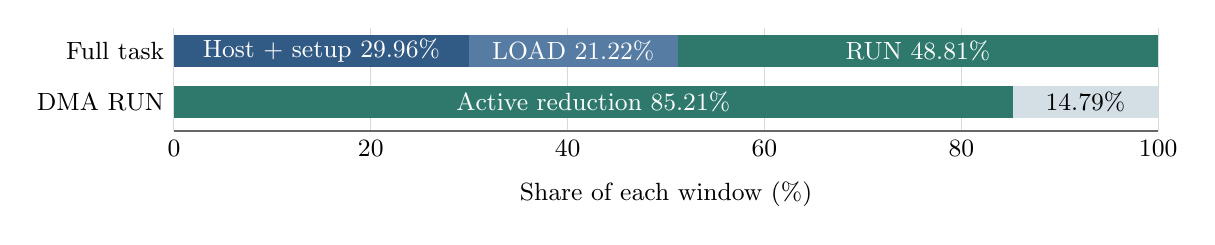
\begin{tikzpicture}[x=.125cm,y=.9cm,font=\small]
\foreach \x in {0,20,40,60,80,100}{
  \draw[black!15] (\x,.10) -- (\x,1.55);
  \node[below] at (\x,.10) {\x};
}
\fill[hostblue] (0,1) rectangle (29.956,1.46);
\fill[loadblue] (29.956,1) rectangle (51.179,1.46);
\fill[runblue] (51.179,1) rectangle (99.991,1.46);
\fill[idlegray] (99.991,1) rectangle (100,1.46);
\fill[runblue] (0,.28) rectangle (85.207,.74);
\fill[idlegray] (85.207,.28) rectangle (100,.74);
\node[left] at (0,1.23) {Full task};
\node[left] at (0,.51) {DMA RUN};
\node[white] at (14.978,1.23) {Host + setup 29.96\%};
\node[white] at (40.567,1.23) {LOAD 21.22\%};
\node[white] at (75.585,1.23) {RUN 48.81\%};
\node[white] at (42.604,.51) {Active reduction 85.21\%};
\node at (92.604,.51) {14.79\%};
\node at (50,-.80) {Share of each window (\%)};
\draw[black!60] (0,.10) -- (100,.10);
\end{tikzpicture}
\end{document}
